\section{Fundamentos Teóricos}

Nesta seção, serão apresentados as fórmulas básicas ao entendimento do
funcionamento de um circuito. Além de apresentar conceitos importantes.

\subsection{\textbf{O que é um circuito elétrico}}

Circuito elétrico, nada mais é do que um interconexão de elementos elétricos.
Elementos esses que são os componentes que formam tal circuito.

\subsection{\textbf{Grandezas importantes}}

Aqui uma tabela demosntrando as grandezas e unidades mais importantes para o
tema tratado no documento:
\newline

\begin{table}[H]
	\centering
	\caption{Grandezas e Unidades Básicas do SI}
	\begin{tabular}{m{3cm}m{2cm}m{1.5cm}}
		\hline
		\textbf{Quantidade}       & \textbf{Unidade básica} & \textbf{Símbolo} \\
		\hline
		Comprimento               & metro                   & m                \\ \hline
		Massa                     & quilograma              & kg               \\ \hline
		Tempo                     & segundo                 & s                \\ \hline
		Corrente elétrica         & ampère                  & A                \\ \hline
		Temperatura termodinâmica & kelvin                  & K                \\ \hline
		Intensidade luminosa      & candela                 & cd               \\ \hline
		Carga                     & coulomb                 & C                \\ \hline
	\end{tabular}
\end{table}

\subsection{\textbf{Grandezas importantes}}

Sabe-se que toda matéria é formada por elementos fundamentais --- átomos,
que são contituídos por elétrons, prótons e neûtrons. Vale lembrar também da
carga \textit{e} ser \( -1.602 \times 10^{-19} \)C e que quando temos o mesmo
número de prótons e elétrons temos um átomo de carga neutra.

\subsection{\textbf{Noções básicas}}

Sendo as cargas elétricas móveis, devemos considerar o fluxo destas. Portanto
quando um fio condutor é ligado a uma bateria, as cargas positivas devem se
mover para uma direção e as negativas para a direção oposta. Por convenção o
fluxo da corrente é aquele das cargas positivas ou oposta as negativas. Conforme
Figura~\ref{fig:fig1}.

\begin{figure}[H]
	\centering
	\setlength{\fboxsep}{0pt}
	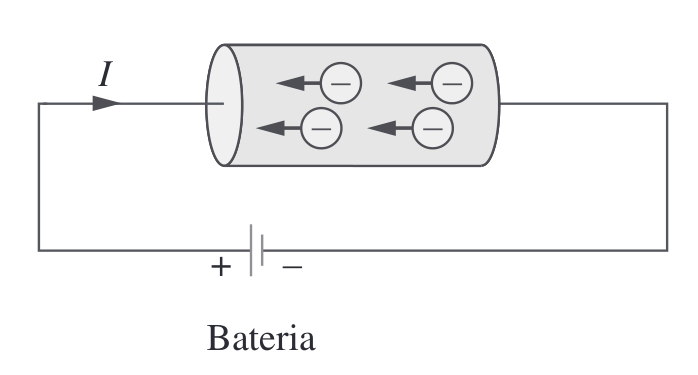
\includegraphics[height=0.1\textwidth]{./fig/fig1.png}
	\caption{Corrente elétrica devido ao fuxo de cargas eletrônicas em um condutor.}
	\label{fig:fig1}
\end{figure}
